\section{\Tool{}'s design}
\label{sec:design}

We now discuss \tool{}'s design.  We start by laying out the involved parties
and their trust assumptions (\S~\ref{sec:trust-assumptions}), followed by an
overview of our system (\S~\ref{sec:overview}).  We then discuss the two major
aspects of our tool kit: the build system (\S~\ref{sec:build-system}) and
\tool{} itself~(\S~\ref{sec:framework}).

\subsection{Trust assumptions}
\label{sec:trust-assumptions}

Our setting has three participants that have the following trust assumptions:
%
The \emph{service provider} runs a service for its clients.  As part of its
operations, the service provider wants to process sensitive client information.

The \emph{client} is a user of the service provider.  It does not trust the
service provider with its sensitive information and demands verifiable
guarantees that the service provider will never see the client's sensitive
information in plaintext.

The \emph{enclave provider} makes available enclaves to the service provider.
Both the client and the service provider trust that the enclave provider's
enclaves have the advertised security attributes of integrity, confidentiality,
and verifiability.

\subsection{Design overview}
\label{sec:overview}

We begin with an informal overview of \tool{} to provide intuition.  Subsequent
sections elaborate on this high-level picture.  The life cycle of an enclave
application that uses \tool{} involves five steps:

\begin{enumerate}
    \item The service provider wants to run an existing service in an enclave.
      Assuming that the service builds reproducibly, the service provider then
      publishes the service's source code for its clients to audit.

    \item The service provider bundles its service with \tool{} and launches the
      enclave, which is now ready to receive incoming connections.

    \item Users audit the service's source code.  Once a user is convinced that
      the code is free of security bugs, she compiles the service using the
      deterministic build system, which results in an image checksum.

    \item The client establishes an end-to-end encrypted network connection with
      the enclave.  Right \emph{after} establishing the secure channel but
      \emph{before} revealing any sensitive information, the client provides a
      nonce and asks the enclave for an attestation document.

    \item The enclave receives the nonce and asks its hypervisor to generate an
      attestation document that contains the client-provided nonce
      \emph{and} the public key that the enclave uses to establish the secure
      channel.  The enclave returns the resulting attestation document (which
      contains the image checksum) to the client.

    \item The client performs various checks (see \S~\ref{sec:attestation} for
      details) and trusts the enclave if all checks pass.  The client is then
      convinced that it's communicating with the code that the user audited in
      the previous steps, and is willing to reveal her sensitive information to
      the enclave.
\end{enumerate}

\subsection{Enabling reproducible builds}
\label{sec:build-system}

Once a user convinced herself of the service's correctness, she compiles the
code to arrive at an image ID---a SHA-384 hash over the enclave image as
discussed in Section~\ref{sec:nitro}.  Crucially, we need a \emph{deterministic
mapping} between the code and its corresponding image ID because the service
provider and clients must agree on the image ID that's running in the enclave.
Docker by itself does not provide a deterministic mapping because---among other
things---Docker records timestamps in its build process, causing subsequent
builds of identical code to result in different image IDs.\footnote{In essence,
a Docker image is an archive of a file system.  A Docker image is reproducible
when separate build processes arrive at the exact same file system, including
meta data like timestamps.}  To obtain reproducible builds, we take advantage of
kaniko~\cite{kaniko}, which has the advantage that one can integrate it easily
into existing Docker-based workflows.  Kaniko's purpose is to build container
images from a Dockerfile while itself in a container but we use kaniko because
it can do so reproducibly.  As long as the client and service provider use the
same source code, kaniko version, and compiler, they can build identical
images---even when compiling the code on different platforms, like Mac OS and
Linux.  Equipped with a locally-compiled image ID, the client is now ready to
interact with the enclave.

\subsection{\Tool{}'s components}
\label{sec:framework}

Having discussed how the client and service provider can independently arrive at
identical image IDs, we now turn to \tool{}'s specific components.  The
following sections discuss how \tool{}
communicates securely with the outside world (\S~\ref{sec:networking});
how we facilitate remote attestation (\S~\ref{sec:attestation});
how enclaves can share their key material to allow for horizontal scaling (\S~\ref{sec:sync});
how to thwart side-channel attacks (\S~\ref{sec:side-channels}); and
how to ingest secrets (\S~\ref{sec:secrets}).
We conclude this section with a simple example (\S~\ref{sec:example}).

\subsubsection{Enabling seamless and secure networking}
\label{sec:networking}

\begin{figure}[t]
  \centering
  \begin{tikzpicture}[node distance=20pt]
	\node [draw,
           label=EC2 parent,
           minimum height=100pt,
           align=center,
           minimum width=80pt] (ec2) {};
	\node [draw,
           label=Enclave,
           right=0pt of ec2,
           fill=black!10,
           minimum height=100pt,
           minimum width=80pt] (enclave) {};
           
    \node [draw,
           below=0pt of enclave.south west,
           minimum width=160pt] (hypervisor) {Hypervisor};
	   
	\node [draw,
           align=center,
           minimum height=25pt,
           yshift=-5pt,
           above=of ec2.south] (viproxy) {TCP proxy};

	\node [draw,
           align=center,
           yshift=5pt,
           below=of ec2.north] (socks) {SOCKS\\proxy};
  
	\node[draw,
          align=center,
          fill=white,
          minimum height=25pt,
          yshift=-5pt,
          above=of enclave.south] (app) {Application};
	      
	\node [draw,
           minimum height=16pt,
           yshift=35pt,
           left=of ec2.west] (backend) {Back end};

    \node [draw,
           below=of backend] (letsencrypt) {Let's Encrypt};

    \node [draw,
           below=of letsencrypt,
           minimum height=16pt] (client) {Client};

    \node [right, align=center, rotate=90] at (enclave.west) {\footnotesize \color{gray} VSOCK\\\footnotesize \color{gray} interface};

    % Application asks the hypervisor for randomness.
    \draw[-latex] (app.south) -- ([xshift=40pt]hypervisor.north)
        node [midway, fill=white, circle, inner sep=0pt] {\ding{202}};

    % Application talking to Let's Encrypt.
    \draw[-latex, densely dotted] ([yshift=10pt]app.west) -- ([yshift=10pt]viproxy.east)
        node [midway, fill=white, circle, inner sep=0pt] {\ding{203}};
    \draw[-latex, densely dotted] ([xshift=-3pt]viproxy.north) -- ([xshift=-3pt]socks.south);
    \draw[-latex, densely dotted] ([yshift=-3pt]socks.west) -- ([yshift=3pt]letsencrypt.east);

    % Let's encrypt probing Application.
    \draw[-latex, densely dashdotted] ([yshift=-3pt]letsencrypt.east) -- ([yshift=3pt]viproxy.west)
        node [midway, fill=white, circle, inner sep=0pt] {\ding{204}};
    \draw[-latex, densely dashdotted] ([yshift=3pt]viproxy.east) -- ([yshift=3pt]app.west);

    % Clients talking to the application.
    \draw[-latex] (client.east) -- ([yshift=-3pt]viproxy.west)
        node [midway, fill=white, circle, inner sep=0pt] {\ding{205}};
    \draw[-latex] ([yshift=-3pt]viproxy.east) -- ([yshift=-3pt]app.west);
    
    % Application talking to backend.
	\draw[-latex, densely dashed] ([yshift=-10pt]app.west) -- ([yshift=-10pt]viproxy.east)
	    node [midway, fill=white, circle, inner sep=0pt] {\ding{206}};
	\draw[-latex, densely dashed] ([xshift=3pt]viproxy.north) -- ([xshift=3pt]socks.south);
	\draw[-latex, densely dashed] ([yshift=3pt]socks.west) -- (backend.east);
\end{tikzpicture}
  \caption{Upon bootstrapping, the application first asks the hypervisor for
    randomness to seed its entropy pool (\ding{202}), followed by initiating an
    ACME session to obtain a Let's Encrypt-signed certificate (\ding{203}), after
    which clients can establish HTTPS connections with the enclave (\ding{204})
    and the enclave can forward data to its back end (\ding{205}).  All of the
    application's ingress and egress  traffic is routed over a TCP proxy that
    translates between AF\_INET and AF\_VSOCK.}
  \label{fig:networking}
\end{figure}

Nitro enclaves have no networking interface.  Their only way to talk to the
outside world is a VSOCK interface that's connected to the EC2 host.  \Tool{}
works around this limitation by creating a TAP interface~\cite{tun-tap} inside
the enclave as illustrated in Figure~\ref{fig:networking}.  The TAP interface is
a virtual networking interface that acts as a network bridge between the enclave
and the EC2 host.  This interface routes traffic to a cooperating proxy
application running on the EC2 host, which provides the enclave application with
seamless Internet connectivity for both IPv4 and IPv6.  The proxy supports port
forwarding to both \tool{} and the enclave application, allowing clients to talk
directly to either.  \Tool{} supports two ways for the enclave application to
receive connections from clients:

\begin{description}
  \item[Indirect] \Tool{} acts as an HTTP reverse proxy and forwards incoming
    HTTP requests to the enclave application.  \Tool{} terminates the TLS
    connection, meaning that the enclave application can speak plain HTTP.  This
    mode is only applicable if the enclave application exposes an HTTP API.

  \item[Direct] The enclave application receives incoming connections directly
    from the proxy.  \Tool{} is not involved.  This is useful for enclave
    applications that speak protocols other than HTTP, or require greater
    flexibility than what the reverse proxy provides.
\end{description}

Having established how the enclave application can send and receive network
packets, we now turn our attention to secure channels; specifically: how can we
let clients establish a secure channel that is terminated inside the enclave?

Enclave applications that receive connections directly must implement their own
secure channel but for enclave applications that take advantage of \tool{}'s
reverse proxy, \tool{} offers a secure channel in the form of HTTPS.  When the
enclave first starts, \tool{} fetches a CA-signed certificate from Let's Encrypt
using the ACME protocol~\cite{acme-protocol} and its TLS-ALPN-01
challenge~\cite{tls-alpn} (step~\ding{203}).\footnote{Unlike the DNS-01 and the
HTTP-01 challenge, TLS-ALPN-01 works entirely in the context of TLS and does not
rely on other ports or protocols, which simplifies deployment.}  Crucially, the
certificate \emph{lives and dies} inside the enclave and its private key cannot
be extracted (or injected) by the service provider because enclaves are sealed
at runtime.
%
The EC2 host can obtain a CA-signed certificate for the same FQDN because the
enclave and the EC2 host share an IP address.  This however is of little use to
the EC2 host because we tie the enclave's certificate to an attestation
document as we will discuss next.

\subsubsection{Authenticating secure channels}
\label{sec:attestation}

Assume a client established a TLS connection with an enclave.  How does the
client know that the TLS session is terminated inside the enclave?  And not by
the EC2 host?  Our trust assumptions state that all parties trust the enclave
provider.  In particular, we use an enclave's attestation document as the root
of trust.  We therefore \emph{authenticate a secure channel by binding it to the
enclave's attestation document}.  By including the service's public key in the
attestation document, clients know that they are talking to \emph{an enclave}.
And by auditing the enclave code and building it reproducibly, clients know that
they are talking to \emph{their trusted enclave}.

We now discuss how we allow clients to retrieve and verify an enclave's
attestation over the Internet because Nitro enclaves only allow for local
attestation.  After the client established a secure channel with the enclave, it
needs to know that (i) the channel it just established is terminated
inside the enclave (instead of by the EC2 host) and (ii) the enclave is
running the code that the user audited in the previous step.  To that end, the
client requests the enclave's attestation document---a hypervisor-signed
document that attests to the container image ID that the enclave is running.
To request an attestation document, the client provides a \emph{nonce}---a
160-bit random value---whose purpose is to prevent the service provider from
replaying outdated attestation documents.  Phrased differently, the client
provides a nonce to convince itself that it's talking to a live enclave.
\Tool{} exposes an HTTP endpoint that clients use to request an attestation
document.  An example request looks as follows:

\begin{lstlisting}[numbers=none,basicstyle=\small\ttfamily]
curl -i "https://enclave/attestation?nonce=abcd..."
HTTP/2 200
content-type: text/plain; charset=utf-8
date: Fri, 27 Jan 2023 16:58:55 GMT

hEShATgioFkQ9alpbW9kdWxlX2lkeCdpLTA2Y...
\end{lstlisting}

Upon receiving this client request, the enclave requests an attestation document
from its hypervisor via an \texttt{ioctl} system call, which makes use of
/dev/nsm, a device that is only available inside the Nitro enclaves.  As
illustrated in Figure~\ref{fig:attestation}, \tool{} asks the hypervisor
to include both the nonce \emph{and} the public key of the enclave's secure
channel in the attestation document and sends the resulting attestation document
to the client.\footnote{If the enclave application uses \tool{}'s reverse proxy,
the public key is a hash over the X.509 certificate; otherwise, it's the public
key of whatever secure channel the enclave application uses.}  Upon receiving
the attestation document, the client then verifies the following in order:

\begin{figure}[t]
  \centering
  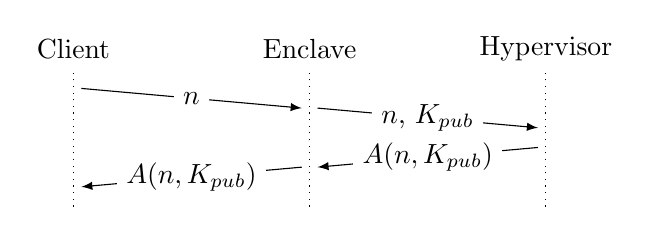
\begin{tikzpicture}[node distance=20pt]

  %               x,y      x,y
  \draw [dotted] (0,0) -- (0,1.75);
  \draw [dotted] (3,0) -- (3,1.75);
  \draw [dotted] (6,0) -- (6,1.75);

  \node at (0,2) {Client};
  \node at (3,2) {Enclave};
  \node at (6,2) {Hypervisor};

  \draw [-latex]
        (0.1, 1.5) -- (2.9, 1.25) node [midway, fill=white, text centered]
        { $n$ };

  \draw [-latex]
        (3.1, 1.25) -- (5.9, 1) node [midway, fill=white, text centered]
        { $n$, $K_{pub}$ };

  \draw [-latex]
        (5.9, 0.75) -- (3.1, 0.5) node [midway, fill=white, text centered]
        { $A(n, K_{pub})$ };

  \draw [-latex]
        (2.9, 0.5) -- (0.1, 0.25) node [midway, fill=white, text centered]
        { $A(n, K_{pub})$ };

\end{tikzpicture}

  \caption{Clients provide a nonce $n$ when requesting an attestation document
  from the enclave.  The enclave asks its hypervisor for the attestation
  document $A$, providing the client's nonce and its public key $K_{pub}$.  The
  hypervisor responds with the attestation document $A(n, K_{pub})$, which the
  enclave forwards to the client.}
  \label{fig:attestation}
\end{figure}

\begin{enumerate}
  \item The attestation document is signed by the AWS root CA whose public key
    (which serves as the root of trust) is known to all parties.  This prevents
    all parties except Amazon from issuing malicious attestation documents.
  \item The challenge nonce is part of the attestation document.  This prevents
    adversaries from replaying old attestation documents.
  \item The fingerprint of the enclave's X.509 certificate from the TLS session
    is part of the attestation document.  This prevents adversaries from
    intercepting the secure channel.
  \item The enclave's image ID is identical to the image ID that the client
    compiled locally.  This prevents adversaries from tricking clients into
    talking to a malicious enclave.
\end{enumerate}

Only if all four conditions hold is the client convinced that it is talking to
an enclave running the previously-audited code \emph{and} that the secure
channel is terminated inside the enclave.  Note that the EC2 host is able to
intercept the secure channel with its own CA-signed certificate but clients will
only trust the EC2 host if (and only if) it can present an attestation document
that is valid for the enclave image, which it can't because it is unable to
spoof the AWS root CA signature that authenticates the attestation document.
The only way for the EC2 host to obtain such an attestation document is to spawn
an enclave that runs the exact code that the client is expecting---and it
already does exactly that!  Now that the client has established a trust
relationship with the enclave, it is ready to reveal sensitive information to
the enclave.

The hypervisor can generate attestation documents quickly (cf.
\S~\ref{sec:attestation-performance}) but they do require an extra round trip
between the client and the enclave before the client is willing to reveal
sensitive information: the client first provides a nonce to the enclave and the
enclave responds with an attestation document.  To eliminate future round trips,
clients can pin the enclave's public key once they verified the attestation
document.

% \paragraph{Manual client-side verification}
% 
% In general, we envision that remote attestation is handled transparently by
% client software, without involving the user.  In some cases however, users may
% wish to manually verify an enclave.  Even for developers, remote attestation is
% a complex process that is difficult to understand and work with.  To make
% matters more complex, in our setting end users are expected to conduct remote
% attestation.  We therefore made a careful effort to abstract away technical
% details.  A user wishing to remotely verify an enclave essentially asks herself
% ``does the enclave that's exposed at a given URL run the source code that I just
% audited?''  We built a tool set that reduces the process to the running of a
% Makefile,\footnote{The source code is available at:
% \url{https://github.com/brave-experiments/verify-enclave}.} i.e.:
% 
% \begin{lstlisting}[numbers=none,basicstyle=\small\ttfamily]
% make verify CODE="/path/to/enclave/code/" \
%             ENCLAVE="https://example.com/attest"
% \end{lstlisting}
% 
% The first argument, \texttt{CODE}, points to the directory containing the source
% code that the enclave is supposedly running, and the user audited.  The second
% variable, \texttt{ENCLAVE}, points to the URL endpoint of the enclave that the
% user's client is connecting to.  When the user runs this command, the Makefile
% deterministically compiles the given source code to obtain its image ID, asks
% the enclave for an attestation document, verifies the document, and ensures that
% the attestation document is for the image ID that was compiled in the first
% step.  If all checks pass, the tool informs the user accordingly.

\subsubsection{Syncing key material among enclaves}
\label{sec:sync}

Enclaves are sealed at runtime, preventing anyone (including both Amazon and the
service provider) from extracting key material that was generated inside the
enclave.  While a desirable property, this complicates horizontal scaling.  If a
single enclave proves unable to handle traffic load, one must scale horizontally
by starting new enclaves.  In some applications, it is unacceptable for each
enclave to use distinct key material.  Instead, enclaves must synchronize their
key material to appear to the outside world like a single machine.  While it is
possible to accomplish key synchronization using tools like the AWS key
management service (KMS),\footnote{One could encrypt the keys using a KMS policy
that dictates that only enclaves are allowed to decrypt it, and store the
encrypted key in a location that all enclaves can access, e.g., an S3 bucket.}
we refrain from using KMS because there is no way for users to verify that the
service provider configured KMS as promised.  We therefore devise a novel,
user-verifiable protocol that enables key synchronization without having to rely
on external services.

We solve this problem in two steps: \emph{discovery} and \emph{synchronization}.
First, enclaves must be able to discover each other, i.e., learn each other's IP
addresses.  Then, enclaves can establish connections with each other and
initiate key synchronization.  Our protocol dictates that when a new enclave
bootstraps, it first tries to discover already-existing enclaves.  If there are
none, the enclave knows that it is the ``origin'' enclave.  It then generates
new key material that it will share with future enclaves.  If however it
discovers other enclaves, the new enclave establishes a connection with another,
randomly-chosen enclave and initiates key synchronization.  Crucially, key
material is only shared after \emph{mutual attestation}, i.e., the origin and
new enclaves verify each other, and exchange key material only if remote
attestation succeeds.  Key synchronization happens in three steps, as
illustrated in Figure~\ref{fig:key-synchronization}.

\begin{figure}[t]
  \centering
  \begin{tikzpicture}[node distance=20pt]

  \node [draw,
         align=center,
         fill=black!20!gray,
         minimum height=70pt] (enclave2) {\color{white}New\\\color{white}enclave};
  \node [draw,
         align=center,
         fill=black!20!gray,
         minimum height=70pt,
         right=140pt of enclave2] (enclave1) {\color{white}Original\\\color{white}enclave};
  \node [draw,
         densely dotted,
         label=below left:Virtual network,
         fit=(enclave1) (enclave2)] {};

  \node [draw,
         above=of enclave2] (resolver) {DNS resolver};

  % New enclave discovers existing enclaves via DNS.
  \draw [-latex] ([xshift=3pt]enclave2.north) -- ([xshift=3pt]resolver.south)
        node [midway, right] {Request DNS SRV records};
  \draw [latex-] ([xshift=-3pt]enclave2.north) -- ([xshift=-3pt]resolver.south);

  % New enclave asks original enclave for nonce.
  \draw [-latex] ([yshift=30pt]enclave2.east) -- ([yshift=25pt]enclave1.west)
        node [midway, fill=white, align=center]
        {\emph{Request nonce}};
  \draw [latex-] ([yshift=15pt]enclave2.east) -- ([yshift=20pt]enclave1.west)
        node [midway, fill=white, align=center]
        {$\textrm{nonce}_o$};

  % New enclave asks for keys.
  \draw [-latex] (enclave2.east) -- ([yshift=-5pt]enclave1.west)
        node [midway, fill=white, align=center]
        {\emph{Request keys}\\$A_{n}(\textrm{nonce}_o, K_n, \ \textrm{nonce}_n$)};

  \draw [latex-] ([yshift=-30pt]enclave2.east) -- ([yshift=-25pt]enclave1.west)
        node [midway, fill=white, align=center]
        {$A_{o}(\textrm{nonce}_n, \textsf{Enc}(K_n, s))$};

\end{tikzpicture}

  \caption{When a new enclave bootstraps, it discovers existing enclaves by
    obtaining the DNS SRV record for its own, hard-coded FQDN.  The enclave then
    initiates key synchronization by first requesting a nonce.  Then, the new
    enclave requests the origin enclave's key material by submitting its own
    attestation document, followed by receiving the origin enclave's attestation
    document, which contains encrypted key material.}
  \label{fig:key-synchronization}
\end{figure}

\begin{enumerate}

  \item Once a new enclave is spun up, it queries the DNS SRV record of the FQDN
    that is hard-coded in the enclave, e.g., example.com.  The DNS resolver will
    return the record, containing a list of enclaves that are already running
    and initialized.  The new enclave picks a random enclave from the list and
    initiates key synchronization.

  \item The new enclave asks the existing enclave for a random nonce,
    $\textrm{nonce}_o$.  Each enclave caches $\textrm{nonce}_o$ for only one
    minute to mitigate denial-of-service attacks.

  \item The new enclave now requests the key material from the existing enclave.
    As part of the request, it provides its attestation document that contains
    $\textrm{nonce}_o$ (to prove freshness to the existing enclave);
    $\textrm{nonce}_n$ (the existing enclave is expected to add this nonce to
    its attestation document); and $K_n$ (a NaCl public key~\cite{nacl} to which
    the key material should be encrypted).  Upon receipt of the new enclave's
    attestation document, the existing enclave verifies the attestation
    document's signature and ensures that the new enclave is running the same
    code, i.e., the image ID that uniquely identifies the enclave
    image is identical.  Once the existing enclave is convinced that it is
    dealing with a genuine new enclave, it creates an attestation document by
    including $\textrm{nonce}_n$ (to prove freshness to the new enclave) and
    $\textsf{Enc}(K_n, s)$---the key material $s$ is encrypted using the public
    key that the new enclave provided in the request.  Finally, the new enclave
    verifies the attestation document, decrypts the key material, and uses it to
    finish bootstrapping.

\end{enumerate}

% Security considerations.
The security of key synchronization is paramount.  We take advantage of mutual
remote attestation to protect the key material.  As an optional layer of
defense-in-depth, synchronization should be configured to use a private network,
which prevents arbitrary Internet hosts from talking to the synchronization
endpoint.  Kubernetes can provide a private network and is an attractive
component in our setting considering that enclave applications are essentially
compiled Docker images, which Kubernetes manages.

In their 2022 USENIX Security paper, Chen and Zhang present MAGE, a protocol
that allows enclaves to mutually verify each other without relying on a trusted
third party~\cite{Chen2022a}.  We could have built key synchronization on top of
MAGE but found that our setting is considerably simpler because only
\emph{identical} enclaves request each other's key material, eliminating the
need for the more flexible---but also more complex---MAGE protocol.

\subsubsection{Side-channel attacks}
\label{sec:side-channels}

The enclave's parent EC2 host cannot see \emph{what} clients send to the enclave
but it can see \emph{how much} clients send and \emph{how long} it takes the
enclave to process data.  The EC2 host can exploit these side channels to learn
more about the client's confidential information and computation.  While such
side channels must be avoided, \tool{} is not the place to do so.  Instead, it
is the application developer's responsibility to identify and address this class
of attacks.  Section~\ref{sec:applications} introduces two applications and
discusses side channel attacks in their respective setting.  Similarly out of
scope are programming bugs in the enclave application.  Memory corruption bugs
may be more difficult to exploit in an enclave application\footnote{The
untrustworthy operating system (which may be under attacker control) is
prohibited by hardware to read the enclave application's memory or registers in
clear text, which forces the attacker to operate blindly.} but Lee et al.
adapted a return-oriented programming attack against SGX to show that such
attacks are practical~\cite{Lee2017a}.

\subsubsection{Ingesting secrets}
\label{sec:secrets}

A key design requirement of \tool{} is that users must be able to audit the
enclave application's code.  The service provider is therefore unable to hide
any software configuration from the user.  Service providers can work around
this shortcoming by exposing an authenticated HTTP handler that take as input
arbitrary data that updates the enclave's state.  Consider a system that takes
as input client IP addresses, anonymizes them, and forwards the anonymized
addresses to a back end (cf. \S~\ref{sec:tokenization}).  The service provider
now wants to compare submitted IP addresses to a confidential deny list.  If
however the deny list is hard-coded in the publicly available enclave
application, it is readily visible to anyone.  The service provider can solve
this problem by adding to the enclave application a new HTTP handler that takes
as input the confidential data it seeks to protect from the users' eyes.  Once
the enclave is running, the service provider loads the confidential data at
runtime, by calling the end point.  To prevent users from submitting bogus data,
the endpoint must be authenticated, i.e., the code could hard-code the service
provider's public key and only accept data that carries a valid signature of the
service provider's private key.

This technique for ingesting secrets is flexible---so flexible, in fact, that
the service provider could abuse it to ingest code at runtime, which would
nullify the enclave's verifiability requirement.  Vigilant users would never
trust an enclave whose code can change at runtime.  We therefore argue that an
HTTP handler for the purpose of ingesting secrets must be constrained to a point
that only data of a well-defined type can be ingested.

\subsubsection{An example}
\label{sec:example}

Figure~\ref{fig:example} illustrates how an enclave application (called
\texttt{enclave-app}) can run alongside \tool{}.  Figure~\ref{fig:dockerfile}
shows a Dockerfile that adds \tool{}, the enclave application, and a start
script to the image, followed by launching the start script, which is
illustrated in Figure~\ref{fig:start}.  All the script does is first launch
\tool{} in the background followed by launching the enclave application.  If
the application builds reproducibly, it is possible to run it inside an enclave
\emph{without modifications}.

\begin{figure}[t]
  \begin{subfigure}[b]{\linewidth}
    \centering
    \begin{lstlisting}
    FROM alpine:latest

    COPY nitriding /bin/
    COPY enclave-app /bin/
    COPY start.sh /bin/

    CMD ["start.sh"]
    \end{lstlisting}
    \caption{A Dockerfile that embeds \tool{} along with the enclave
      application, \texttt{enclave-app}.}
    \label{fig:dockerfile}
  \end{subfigure}

  \begin{subfigure}[b]{\linewidth}
    \centering
    \begin{lstlisting}[language=bash]
    #!/bin/sh

    # Launch nitriding in the background.
    nitriding \
      -fqdn "example.com" \
      -acme \
      -appwebsrv "http://127.0.0.1:8080" &

    # Launch the application.
    enclave-app
    \end{lstlisting}
    \caption{The start.sh shell script launches \tool{} in the background,
    followed by launching the enclave application}
    \label{fig:start}
  \end{subfigure}

  \caption{An example of how a simple enclave application can be bundled with
  \tool.}
  \label{fig:example}
\end{figure}
